\documentclass[UTF8,a4paper]{ctexart}
\usepackage[utf8]{inputenc}
\usepackage{amsmath}
\usepackage{pdfpages}
\usepackage{graphicx}
\usepackage{wrapfig}
\usepackage{listings}
\usepackage{multicol}
\newcommand{\tabincell}[2]{\begin{tabular}{@{}#1@{}}#2\end{tabular}}
\title{智能交通仿真平台程序说明}
\author{张蔚桐\ 2015011493\ 自55}
\begin {document}
\maketitle
\clearpage
\section{程序架构}
\begin{figure}
\centering
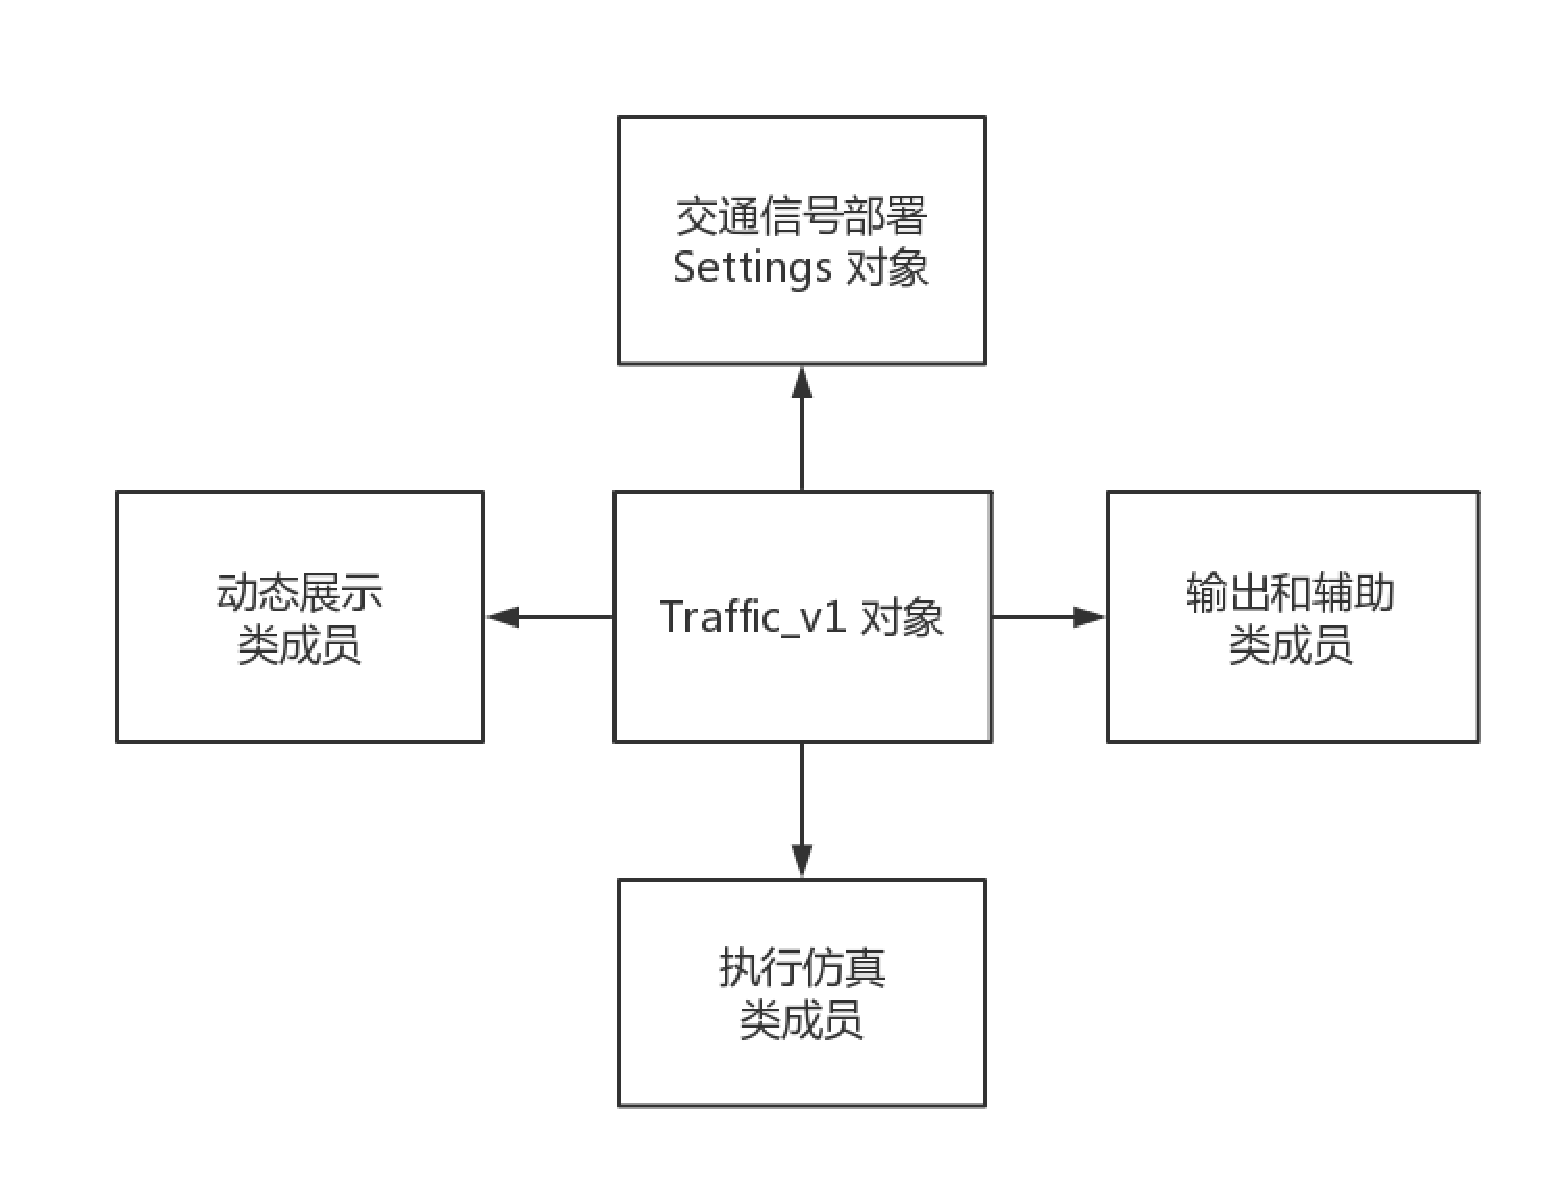
\includegraphics[width=\textwidth]{ClassDiagram.eps}
\caption{主体程序架构}
\label{Trafficv1}
\end{figure}
整个程序使用C++/Qt进行开发,核心由一个Traffic\_v1对象构成,这个对象的UML图如图(\ref{Trafficv1})所示

其中大致可以分为以下几个模块
\clearpage
\subsection{显示模块}
这些类成员主要为用户界面显示和调整设计,其中包括
\begin{multicols}{2}
\begin{lstlisting}[language=C++]
QPushButton* end;
QPushButton* edit;
QRadioButton* fast;
QRadioButton* medium;
QRadioButton* slow;
QRadioButton* very_slow;
QLabel* speed;
QLabel* ratio;
QSlider* ratio_setting;
QLabel* ratio_shower;
com_label* st;
com_label* _st;
QSlider* A_L;
QSlider* B_L;
QSlider* C_L;
QSlider* D_L;
QLabel*A_A;
QLabel*B_A;
QLabel*C_A;
QLabel*D_A;
QLabel*A_B;
QLabel*B_B;
QLabel*C_B;
QLabel*D_B;
\end{lstlisting}
停止按钮 \\
信号部署编辑 \\
快速(1000倍速) \\
中速(100倍速) \\
低速(10倍速) \\
极低速(1倍速)(仅用于debug) \\
“speed”标签\\
“Ratio Controled”标签\\
设置控制车辆比例的滑动条\\
显示控制车辆比例的标签\\
统计信息的类别的显示栏(12个)\\
统计信息的数据显示栏(12个)\\
设置车流量的滑块(W方向)\\
设置车流量的滑块(S方向)\\
设置车流量的滑块(E方向)\\
设置车流量的滑块(N方向)\\
W方向标签\\
S方向标签\\
E方向标签\\
N方向标签\\
W方向车流量数值显示\\
S方向车流量数值显示\\
E方向车流量数值显示\\
N方向车流量数值显示\\
\end{multicols}

程序每向前执行一步仿真就进行一次显示上的刷新,并将其绘制在左侧的交通信号口中,具体的实现见"paint.cpp",整个函数完成如下步骤
\begin{enumerate}
\item 绘制十字路口基本单元
\subitem 根据信号配时的部署绘制红绿灯
\subitem 绘制交通路口车道线
交通线显示长度为30m,宽度为当前标准宽度(六车道22.5m)
\item 绘制来车和离开的车辆

其中,开往交通路口的车辆可以接受控制,而驶出交通路口的车辆程序认为他们已经不必接受控制,并为他们自行补足了相关驾驶策略
\item 绘制交通路口内轨迹线

程序中没有处理车辆在交通路口内的行为,因此采用轨迹线代替车辆的具体位置。其中,当车辆进入交通路口后,我们认为左转,直行,右转车辆驶离交通路口的时间分别为3s,2s和1s,这些参数可以在simulate函数中进行相关的修改。而相应的轨迹线将持续对应的时间

可以认为,轨迹线的交叉次数是交通路口内混乱程度的表述,如果存在着过多的交叉次数,可能会影响交通路口的通行效率以及造成危险,但这主要是信号配时的问题
\end{enumerate}
\subsection{仿真模块}
这是程序执行的核心模块,按照前文仿真速度设置控件设置的仿真速度(快,中,慢以及极慢)提供一个间隔为1ms,10ms,100ms以及1000ms的触发信号QTimer*timer;

接受触发信号之后,程序按照如图(\ref{timeflow})执行相关的操作

在执行流程中,进程控制块决定是否自动停止仿真(根据是否满足用户的停止仿真条件等),新车辆生成在每条车道上按照设计的算法生成车辆,用户策略配置将用户策略应用到即将驶入交通岗的每一台车辆上,而系统策略负责处理驶出交通岗的车辆以及某些处于边际情况的车辆。以上的策略,主要改变的是车辆的加速度,接下来的运动学仿真,根据车辆的加速度和速度,决定车辆下一个时刻的位置和速度。最终处理已经驶入交通路口或者即将完全驶出关心的范围的车辆。最终完成系统界面的重绘工作,并等待下一个触发信号的到来。

根据目前程序的执行情况,在100倍速(10ms)下,系统的负担是比较合适的,同时仿真数据也比较稳定,在1000倍速情况下可能出现一些时序上的问题
\begin{figure}
\centering
\includegraphics[width=\textwidth]{TimeFlow.png}
\caption{控制流程}
\label{timeflow}
\end{figure}
\subsection{输出和辅助模块}
这部分模块的主要工作在于将实时的仿真结果输出,其中的一部分在仿真过程图(\ref{timeflow})中,在系统重绘时调用,一部分随着仿真的进行,出现相关情况的边际执行。

随着仿真的进行,系统会建立四张csv表,存储在可执行文件(.exe)目录的根目录下的result文件夹中,result文件夹中的每一个文件夹的命名规则为

\centerline{\textbf{"具体日期+具体时间+仿真模式选择"}}

其中仿真模式选择的具体值将在后文算法设计中提到

四张表分别记录了不同类型的数据
\begin{enumerate}
\item car.csv

这张表记录了每辆车的初始速度(init\_velocity),理想到达时间(thoritical\_time),实际到达时间(act\_time)以及后两者的差值(delta),其中,理想到达时间表示为车辆以初始速度以最大加速度加速到最大限速,之后保持匀速直线运动状态直到驶入交通路口内部所花费的时间,实际时间是车辆经过这段路程实际花费的时间,他们的差值可以理解为车辆在路上浪费的时间
\item stop.csv

这张表记录了每个时刻每个车道停车的总数和系统内停车的总次数,以及占总车辆数的比例。

\item road.csv

这张表记录了每个时刻驶出某条车道的车辆总数和离开系统的车辆总数,以及他们的平均值
\item stop\_time.csv

这张表记录了每个时刻每个车道停车的总时间和系统内停车的总时间,以及分摊到每个车辆上的停车时间。
\end{enumerate}

一般来说,road.csv用来观测整个仿真过程是否正常,而剩余三张表用来评价整个策略的优劣

其中,停车次数按照车辆的速度低于某一设定阈值来确定,停车时间随着车辆的停车不断累加,而停车次数不随车辆的长期停车而改变

\subsection{交通灯设置模块}

交通灯设置模块完成自主定义交通灯的用户需求,其中三个按键“set red/green/yellow behind”完成的是对黑色时间线后面所有时间的选中的信号的设定。同时,此界面可以完成周期的设定,通过移动时间线或指定时间线位置,反复选中要更改的车道,设置信号相位等方式,可以完成没有限制的对周期执行的红绿灯信号的设置。同时,左侧界面会提示当前(黑色时间线时刻)可能在交通路口中出现的轨迹线,提示用户尽可能避免轨迹线的交叉等问题,帮助用户进行更合理的信号配时工作
\section{算法简述}
\subsection{程序基本参数和假定}
程序中认为车辆的最大加速度为$a_{max}$,并且普遍试用于加速过程和刹车过程,同时道路的最高限速为$v_{max}$,最低限速为$v_{min}$

不论哪种策略,如果给出的加速度大于最大加速度,或者计算得到的速度大于最大限速或小于最低限速,程序都会自动将这些值设置为边界值,当遇到红灯情况时,车辆的最小通行速度为0,描述可能存在的停车行为,但是不允许出现倒车的行为。

另外,我们设定期望的引导速度是最高限速的80\%

为简化流程,我们认为车辆在行驶的过程中没有变道行为,这一点在实际生活中也是可以接受的,受到驾驶习惯和交通法规的限制,车辆在即将进入交通路口之前一般会提前完成变道行为,因此我们可以认为在我们控制的区域内车辆的变道行为都已经完成了。因此这点假设是合理的,同时,单单从通行效率的角度来看,变道行为只能降低平均的通行效率,因此作为一个主要的效率进行考察的平台,我们不考虑变道的情况。
\subsection{车辆生成算法}
平台统一假定车辆的到达过程近似是一个泊松过程,同时对这个过程加以一定的限制和调整。

对于一个方向的车流量,通过前面所述的车流量调整滑块设置了平均每小时车流量之后,这个方向上的车辆就将按照这个指定的强度生成车辆。生成车辆后,考虑车辆属于哪个车道,我们认为车辆等可能的出现在任何一个安全车道内,安全车道的意义为车道内的最后一辆车距离车辆生成的位置大于安全距离$S$,如果没有这种安全车道,则这辆车在生成队列中等待,直到出现一个合适的安全车道。

具体的车辆生成算法请参见“Traffic\_v1.cpp”文件中的generate()函数,车辆的生成工作在每一个仿真周期的第二步进行,紧随进程控制模块。
\subsection{路口排队的产生和消散}
为解决路口排队的问题,在路口引入队列car\_block,并且根据当前的信号相位和队列的情况,对后面来车进行如下基本策略控制(即,所有的策略都应满足这些条件)

\begin{enumerate}
\item 红灯

路口中没有进入排队的第一辆车辆按照队尾车辆的位置之后的安全距离$S$为停车位置进行刹车,如果队伍为空,第一辆车辆按照设定的停车线进行刹车。

\item 绿灯

路口中第一辆没有进入排队的车辆在其行驶过程中不能超过队尾车辆的位置之后的安全距离$S$
\end{enumerate}
同时,这个等待队列按照如下的方式进行增长和消散
\begin{enumerate}
\item 增长

如果有车辆进入队尾车辆之后的安全距离内,则其进入队列(而从路口自由行驶车辆中消失)

\item 消散

绿灯情况下所有队列内的车辆均以恒定速度向前运动,如果超过了停车线则进入路口,队列消散
\end{enumerate}
\subsection{跟驰策略的实现}
这是平台实现的三个策略中描述人工驾驶部分的算法,整个算法对每一个车辆分别执行,并考虑如下几种情况
\begin{enumerate}
\item 前车距离大于控制距离$4S$或为队列中的头车

此时描述车辆的间距较远,不必考虑车辆之间可能存在的干扰,因此车辆按照一个合理的加速度向控制速度(最高速度的80\%)加速

\item 前车距离在控制范围内

此时采用跟驰模型来描述车辆的运动,因为交通路口车辆的运动速度存在着巨大的差异,因此考虑采用线性的跟驰模型,即
\begin{equation}
\begin{aligned}
& S=S_0+cV \\
& a_{n+1}=a_n+\frac{\Delta^2_V}{2(\Delta_S-S)}
\end{aligned}
\end{equation}
其中$\Delta_V,\Delta_S$为正的速度差和距离

\item 前车距离过小

此时先考虑将上式处理后变为
\begin{equation}
\begin{aligned}
& S=S_0+cV \\
& a_{n+1}=a_n-\frac{\Delta^2_V}{2(\Delta_S-S)}
\end{aligned}
\end{equation}
来描述车辆的行为,如果计算得到的加速度的绝对值大于最大加速度,采用$-a_{max}$来代替计算得到的加速度
\end{enumerate}
当出现红灯时,如果车辆已经驶入控制距离4S,采用上文所示的方法进行刹车并进入等待队列中。

同样,当红灯转变为绿灯时,自由行驶队列中的第一辆车按照前面消散队列中的恒定速度进行加速或减速,并带动后面的车辆进行运动。

具体的实现请见"User.cpp"全文,其中部分细节不加赘述
\subsection{无车路协同的自主策略的实现}
本策略基于上个跟驰策略进行了一定程度的更改,设计了考虑红绿灯的自主策略,分别考虑如下几个方面。

\begin{enumerate}
\item 在控制距离内

对于在跟驰距离内的车辆,采用同跟驰策略一样的方式进行处理,这里不加重复说明。
\item 头车或在控制距离外

对于有自由行驶能力,不必考虑前车影响的车辆,考虑处理红绿灯的策略

首先计算车辆到达红绿灯路口的最快时间(以最大加速度加速到最大速度之后保持匀速直线运动)和最慢时间(以最大加速度减速到最小速度之后保持匀速直线运动),确定在这段区间内最早的绿灯时间,如果这段区间内不存在绿灯的时间,则同跟驰策略一样进行自由行驶。

如果在这段区间内存在绿灯的实现,车辆采取加速或减速措施,并以期望在那个确定的绿灯时间通过路口为目标调整自己的速度,这期间,如果受到了前面车辆的影响则回到正常的跟驰模型中
\end{enumerate}
同时,处理红绿灯和路口进入排队的策略也和跟驰策略相同,具体的技术细节可见"st1.cpp"中的实现

总体上说,可以认为这个策略就是跟驰策略考虑对信号相位响应之后的优化版
\subsection{有车路协同的自主策略的实现}
这是一个有车间通信的简单的车路协同版本的策略,策略同样对每一个车辆个体执行一遍

策略从队伍中的头车到最后的车辆依次执行,首先头车确定自己的到达路口的最快时间和最慢时间,同时,同上个策略,选定自己的到达时间。

对于之后的每一个车辆,我们认为他们都可能获得前车的期望到达时间,并从这个时间开始,在自己的可能到达时间间隔内找到一个绿灯的时间,即,前车的期望到达时间永远早于后车的期望到达时间(如果都存在的话)。同时,如果前车到达时间不存在的话,认为后车不受约束的进行到达时间的选择。

之后每个车辆按照自己的预期到达时间为目标调整自己的加速度,同时,如果出现了距离前车过近的情况,采用比较强的加速度进行减速。同时,每个车辆的调整策略均是先变速到一个和预期时间相匹配的速度,然后保持匀速直线运动,因此相关的碰撞不会出现多次,只需一次彻底解决即可。

至于不存在期望到达时间的车辆,他们的策略是先加速到一个比较合适的加速度,之后再红绿灯处停车等待通过,这样尽可能的不给后面的车辆制造障碍。

具体的实现在"st2.cpp"中
\subsection{混合驾驶的策略实现}
我们只对人工驾驶+自主驾驶的情况进行混合驾驶策略,即只对策略I和策略II,策略I和策略III进行混合。同时我们认为对于I,III混合的情况,所有有I驾驶的车辆均是没有预期到达时间的。

在车辆生成算法中按照设定的比例来随机生成相关的车辆,在混合驾驶策略中,根据不同的车辆属性选择不同的驾驶策略进行混合。

具体的实现在"combo.cpp"中
\section{运行结果}
\end{document}
